\documentclass{article}
\usepackage[utf8]{inputenc}
\usepackage[T1]{fontenc}
\usepackage[frenchb]{babel}
\usepackage{lmodern}
\usepackage{hyperref}
\usepackage{amsmath}
\usepackage{amssymb}
\usepackage{mathtools}
\usepackage{color}
\usepackage[usenames,dvipsnames,svgnames,table]{xcolor}
\usepackage{tikz}
\usepackage[cm]{fullpage}
\usepackage{siunitx}
\usepackage{../../../eplcommon}
%(Note à moi-même : il est grand temps que sigsys soit passé. Pour que je dors enfin à une heure convenable.)

\title{Signaux et systèmes : échantillonnage}
\author{Jean-Martin Vlaeminck}
\date{\today}
\begin{document}
\maketitle
\section{Rappel des transformées et de leurs propriétés}

Pour chaque classe de signal correspond une représentation de Fourier adéquate. Les $\hat{X}$ et $\tilde{X}$ sont là uniquement pour les différencier de la notation de la DFT, qu'on note ici $X[k]$ (le livre utilise $\tilde{X}[k]$ pour la DFT, et $X[k]$ pour la (DT)FS).

\begin{enumerate}
	\item $x(t)$ continu, non périodique $\Rightarrow$ transformée de Fourier classique (FT) $X(j\omega)$, continue non périodique.
	\begin{align}
	X(j\omega) &= \int_{-\infty}^{\infty} x(t) e^{-j\omega t} \dif{t} \label{eq:ft_from_xt_def} \\
	x(t) &= \frac{1}{2\pi} \int_{-\infty}^{\infty} X(j\omega) e^{j\omega t} \dif{t} \label{eq:xt_from_ft_def}
	\end{align}

	\item $x(t)$ continu, de période $T$ $\Rightarrow$ série de Fourier classique (FS) $\hat{X}[k]$, discrète et non périodique.
	\begin{align}
	\hat{X}[k] &= \frac{1}{T} \int_{T} x(t) e^{-j k \omega_0 t} \label{eq:fs_from_xt_def} \\
	x(t) &= \sum_{k=-\infty}^{\infty} \hat{X}[k] e^{j k \omega_0 t} \label{eq:xt_from_fs_def}
	\end{align}
	où $\omega_0 = \frac{2\pi}{T}$, pour abréger. On intègre sur une période (de longueur $T$), quelconque (celle qui nous arrange).

	\item $x[n]$ discret, non périodique $\Rightarrow$ transformée de Fourier en temps discret (DTFT) $X\left(e^{j\Omega}\right)$, continue et $2\pi$-périodique en $\Gamma$
	\begin{align}
	X\left(e^{j\Omega}\right) &= \sum_{n=-\infty}^{\infty} x[n] e^{-j\Omega n} \label{eq:dtft_from_xn_def} \\
	x[n] &= \frac{1}{2\pi} \int_{2\pi} X\left(e^{j\Omega}\right) e^{j\Omega n} \label{eq:xn_from_dtft_def}
	\end{align}
	où on intègre de nouveau sur une période, donc sur une longueur de $2\pi$, classiquement de $0$ à $2\pi$, ou de $-\pi$ à $\pi$.

	\item $x[n]$ discret, de période $N$ $\Rightarrow$ série de Fourier en temps discret (DTFS) $\tilde{X}[k]$, discrète et $N$-périodique également.
	\begin{align}
	\tilde{X}[k] &= \frac{1}{N} \sum_{n=0}^{N-1} x[n] e^{-\frac{2kj\pi n}{N}} \label{eq:dtfs_from_xn_def} \\
	x[n] &= \sum_{n=0}^{N-1} \tilde{X}[k] e^{\frac{2kj\pi n}{N}} \label{eq:xn_from_dtfs_def}
	\end{align}
	où on fait la somme sur une période de $N$ échantillons quelconque (celle qui nous arrange) dans les deux cas ; classiquement, de $0$ à $N-1$.
\end{enumerate}

Le facteur chiant est présent lors du calcul des $\tilde{X}[k]$/$\hat{X}[k]$ (pour des signaux périodiques donc), et lors du calcul de $x(t)$ ou $x[n]$ (pour des signaux non périodiques).

\section{Représentation en transformée de Fourier de signaux périodiques}

%\begin{figure}
%	\centering
%	\begin{tikzpicture}
%	\draw[thick, -latex] (-4, 0) -- (4, 0);
%	\draw[thick, -latex] (0, -1.5) -- (0, 1.5);
%	\draw[domain=-3.5:3.5, samples=200] plot(\x, {cos()}
%	\end{tikzpicture}
%\end{figure}

Pour un signal $x(t)$ $T$-périodique, même si sa représentation favorite est la FS, on peut écrire une version en transformée de Fourier en utilisant des impulsions :
\begin{equation}
X(j\omega) = 2\pi \sum_{k=-\infty}^{\infty} \hat{X}_\mathrm{FS}[k] \delta\bigg( \omega - k \underbrace{\frac{2\pi}{T}}_{=\omega_0} \bigg)
\label{eq:fs_to_ft}
\end{equation}
La démonstration est à la section 4.2.1, page 342 du livre. Graphiquement, on prend les coefficients de $\hat{X}[k]$, on les dispose tous les $\omega_0$, on les multiplie par $2\pi$ et on les convertit en impulsions.

Pour un signal $x[n]$ $N$-périodique, on peut aussi trouver une écriture sous forme d'une DTFT :
\begin{equation}
X\left(e^{j\Omega}\right) = 2\pi \sum_{k=-\infty}^{\infty} \tilde{X}_\mathrm{DTFS}[k] \delta\bigg( \Omega - k \underbrace{\frac{2\pi}{N}}_{=\Omega_0} \bigg)
\label{eq:dtfs_to_dtft}
\end{equation}
qui reste $2\pi$-périodique, car les $\tilde{X}_\mathrm{DTFS}[k]$ sont $N$-périodiques. Vérifiez en remplaçant $k$ par $k+N$, puis en remplaçant $\Omega$ par $\Omega+2\pi$ !

\section{Échantillonnage d'un signal continu}

Soit un signal $x(t)$, le \emph{signal original}. Supposons qu'on veuille le traiter sur un ordinateur ; il faut donc prendre des échantillons, espacés d'une durée $T_e$, la \emph{période d'échantillonnage}, dont l'inverse, $\frac{1}{T_e} = f_e$, est la \emph{fréquence d'échantillonnage}, le nombre de fois par seconde que l'on ouvre le dispositif pour qu'il prenne un échantillon (une photo). Cela revient à multiplier le signal de départ $x(t)$ par un peigne de diracs
\[ p(t) = \sum_{n=-\infty}^{\infty} \delta(t - n T_e) \]
ou tout autre variante, si par exemple on échantillonne en $T_0$, $T_0+T_e$\dots. On obtient alors
\begin{equation}
x_\delta(t) = \sum_{n=-\infty}^{\infty} x(nT_e) \delta(t-nT_e)
\label{eq:sampling_xdeltat}
\end{equation}
soit un signal constitué de diracs aux points où on a pris un échantillon. La transformée du peigne de diracs est
\begin{equation}
P(j\omega) =  \frac{2\pi}{T_e} \sum_{k=-\infty}^{\infty} \delta\bigg( \omega - k \underbrace{\frac{2\pi}{T_e}}_{=\omega_e} \bigg)
\label{eq:ft_peigne}
\end{equation}
que l'on obtient en calculant la FS $\hat{P}[k]=\frac{1}{T}$ (c'est un signal $T_e$-périodique), puis en calculant la FT à partir de~\eqref{eq:fs_to_ft} ; on a besoin d'une FT car le signal de départ n'est pas forcément périodique, et on convertit donc la FS en impulsions : on obtient ainsi un autre peigne.

A partir du signal $x(t)$, on obtient le signal $x_\delta(t)$ en transformant en diracs les points $x(nT_e)$. On définit aussi un signal discret, équivalent au signal échantillonné,
\[ x_e[n] = x(nT_e) \]
dont on peut connaitre la DTFT $X_e\left(e^{j\Omega}\right)$.

Comme une multiplication en temporel équivaut à une convolution en fréquentiel (attention au facteur $\frac{1}{2\pi}$ !), on obtient
\begin{align*}
X_\delta(j\omega) &= \frac{1}{2\pi} \int_{-\infty}^{\infty} X(j\gamma) P(j(\omega-\gamma)) \dif{\gamma} = \frac{1}{2\pi} \int_{-\infty}^{\infty} \frac{2\pi}{T_e} \sum_{k=-\infty}^{\infty} X(j\gamma) \delta\left(\omega-\gamma-\frac{2k\pi}{T_e}\right) \dif{\gamma} \\
&= \frac{1}{T_e} \sum_{k=-\infty}^{\infty} \int_{-\infty}^{\infty} X(j\gamma) \delta\left(\omega-\gamma-\frac{2k\pi}{T_e}\right) \dif{\gamma} = \frac{1}{T_e} \sum_{k=-\infty}^{\infty} X\bigg(j\bigg(\omega-\underbrace{\frac{2k\pi}{T_e}}_{=k\omega_e}\bigg)\bigg)
\end{align*}
et donc,
\begin{equation}
X_\delta(j\omega) = \frac{1}{T_e} \sum_{k=-\infty}^{\infty} X\left(j\left(\omega-k\omega_e\right)\right)
\label{eq:sampling_ft_delta_from_ft}
\end{equation}
Le spectre d'origine est à chaque fois répliqué aux multiples de $\omega_e$, la pulsation d'échantillonnage, et est multipliée par la fréquence d'échantillonnage.

Lions un peu la DTFT de notre signal $x_e[n]$ non périodique à une possible FT. Tout signal discret $x[n]$ peut d'ailleurs être considéré comme une version échantillonnée d'un autre signal $x_\delta(t)$ à la période $T_e$. On écrit la FT de notre signal $x_\delta(t)$ défini par~\ref{eq:xdeltat} :
\begin{align*}
X_\delta(j\omega) &= \int_{-\infty}^{\infty} x_\delta(t) e^{-j\omega t} \dif{t} \\
&= \int_{-\infty}^{\infty} \sum_{n=-\infty}^{\infty} x[n] \delta(t-nT_e) e^{-j\omega t} \dif{t} = \sum_{n=-\infty}^{\infty} \int_{-\infty}^{\infty} x[n] \delta(t-nT_e) e^{-j\omega t} \dif{t} \\
&= \sum_{n=-\infty}^{\infty} x[n] e^{-j\omega n T_e} = \sum_{n=-\infty}^{\infty} x[n] e^{-j(\omega T_e) n} \\
&= X_e\left(e^{j \omega T_e}\right) = X_e\left(e^{j\Omega}\right) \Big\rvert_{\Omega = \omega T_e}
\end{align*}
et on définit donc la FT du signal $x_e[n]$, à partir de la DTFT, comme étant
\begin{equation}
X_\delta(j\omega) = X_e\left(e^{j\Omega}\right)\Big\rvert_{\Omega = \omega T_e}
\label{eq:sampling_ft_delta_from_dtft}
\end{equation}
et inversement, la DTFT de $x[n]$ à partir de la FT de $x_\delta(t)$ est
\begin{equation}
X_e\left(e^{j\Omega}\right) = X_\delta\left(\frac{\Omega}{T_e}\right)
\label{eq:sampling_dtft_from_ft_delta}
\end{equation}

Si $x_e[n]$ est $N$-périodique (et donc, si $x_\delta(t)$ est $NT_e$-périodique), on a plutôt
\begin{align}
X_\delta(j\omega) &= \frac{2\pi}{T_e} \sum_{k=-\infty}^{\infty} \tilde{X}_e[k] \delta\left(\omega - \frac{2k\pi}{NT_e}\right) \label{eq:sampling_ft_delta_from_dtfs} \\
&= \frac{2\pi}{N T_e} \sum_{k=-\infty}^{\infty} X_e[k] \delta\left(\omega - \frac{2k\pi}{NT_e}\right) = \frac{2\pi}{N T_e} \sum_{k=-\infty}^{\infty} X_e\left(e^{jk\Omega_0}\right) \delta\left(\omega - \frac{2k\pi}{NT_e}\right) \label{eq:sampling_ft_delta_from_dft}
\end{align}
avec $\tilde{X}_e[k]$ les coefficients de la DTFS de $x_e[n]$, $X_e[k]$ les coefficients de la DFT, et $\Omega_0=\frac{2\pi}{N}$. \eqref{eq:sampling_ft_delta_from_dtfs} découle de la combinaison de~\eqref{eq:dtfs_to_dtft} et~\eqref{eq:sampling_ft_delta_from_dtft} ; \eqref{eq:sampling_ft_delta_from_dft} découle de la section suivante.

\subsection{Échantillonnage d'un signal discret}

Il est aussi possible d'échantillonner un signal $x[n]$, en prenant un échantillon tous les $q$ par exemple :
\[ x_e[n] = x[qn] \]
Dans ce cas, si $X\left(e^{j\Omega}\right)$ est la DTFT du signal $x[n]$, alors la DTFT du signal $x_e[n]$ est
\begin{equation}
X_e\left(e^{j\Omega}\right) = \frac{1}{q} \sum_{m=0}^{q-1} X\left(e^{j(\Omega-\frac{2m\pi}{q})}\right)
\label{eq:sampling_dtft_e_from_dtft}
\end{equation}
avec la même interprétation : le spectre d'origine est répliqué à tous les multiples de $\frac{2\pi}{q}$, et est divisée par la ``période d'échantillonnage'' $q$.

\section{Échantillonnage de la DTFT, zero-padding, et la DFT}

Considérons maintenant un signal $x[n]$ de durée $M$ (càd il n'y a que $M$ échantillons contigu non nuls)\footnote{Encore plus rigoureusement, on a $x[n]=0$ pour $n<0$ ou pour $n\ge M$, avec $x[M-1]\neq 0$ (sinon la durée est de $M-1$ et pas de $M$) et $x[0]\neq 0$ (sinon on décale le signal dans le temps).}. C'est typiquement ce qu'on obtient quand on a échantillonné un signal $x(t)$ et qu'on a pu en enregistré qu'une partie. Comme tout signal discret, ce signal a une DTFT $X\left(e^{j\Omega}\right)$. Seulement voilà, la DTFT est continue et on aimerait bien travailler avec un spectre discret.

Première méthode : échantillonner la DTFT. On prend $N$ échantillons de la DTFT, espacés de $\frac{2\pi}{N}$ :
\begin{equation}
X_\mathrm{DFT}[k] = X\left( e^{\frac{2k\pi j}{N}} \right)
\label{eq:dft_from_dtft}
\end{equation}

Deuxième méthode : on considère une version périodisée du signal $x[n]$
\[ x_{N'}[n] = \sum_{m=-\infty}^{\infty} x[n + mN] \].
Ce signal a une période $N'$, et pour $N'>M$, les échantillons manquant sont pris comme valant zéro (\emph{zero-padding}). On calcule alors la DTFS $\tilde{X}_P[k]$ \footnote{$P$ pour périodisé, notation non officielle} de ce signal périodisé :
\begin{equation}
DTFS = \tilde{X}_P[k] = \frac{1}{N'} \sum_{n=0}^{N'-1} x_{N'}[n] e^{-\frac{2j\pi k n}{N'}}
\label{eq:dtfs_from_x_zero_pad}
\end{equation}

Eh bien, il se fait que lorsque $N=N'$, on a $\tilde{X}_P[k] = \frac{1}{N}X[k]$. On définit la \emph{transformée de Fourier discrète} comme
\begin{equation}
DFT = X[k] = \sum_{n=0}^{N'-1} x_{N'}[n] e^{-\frac{2j\pi k n}{N'}}
\label{eq:dft_def}
\end{equation}

La DFT a donc la propriété d'être un échantillonnage de la DTFT (on en garde $N$ échantillons). Au facteur $N$ près, il s'agit de la DTFS de la version $N$-périodisée du signal $x[n]$. La DFT est donc $N$-périodique, et la iDFT est aussi $N$-périodique. En fait, sans plus d'information, la DFT va considérer que le signal de longueur $N$ qu'on lui passe est $N$-périodique, et va ainsi en ressortir un vecteur $X[k]$ $N$-périodique, à partir duquel on ne pourra que récupérer ce faux signal périodique. Et plus on ajoutera d'échantillons nuls (\emph{zero-padding}), plus la DFT va se rapprocher de la DTFT.

Si le signal $x[n]$ (ou plutôt, $x_e[n]$) était un échantillonnage à la fréquence $1/T_e$ d'un signal $x(t)$, on peut même aller plus loin, en reliant la DFT $X[k]$ à la DTFT de $x_e[n]$, et en reliant la DTFT de $x_e[n]$ à la FT de $x(t)$ et à la FT de $x_\delta(t)$ :
\begin{equation}
DFT = X[k] = X_e\left(e^{j \frac{2\pi k}{N}}\right) = X_\delta\left(j \frac{2\pi k}{N}\frac{1}{T_e}\right) = \frac{1}{T_e} \sum_{m=-\infty}^{\infty} X\left(j\left( \frac{2k\pi}{N T_e} - m \frac{2\pi}{T_e} \right)\right)
\label{eq:dft_dtft_ft_delta_ft_relationships}
\end{equation}

\subsection{Échantillonnage de la FT : la FS}

De la même manière que l'échantillonnage de la DTFT d'un signal discret\footnote{représentant peut-être un signal continu} conduit à la DFT, sorte de DTFS un peu différente, il est possible d'échantillonner la FT d'un signal continu non périodique\footnote{Et non échantillonné, d'ailleurs} et à durée finie $T_0$ $x(t)$. Et qu'est-ce que cela donne ? La série de Fourier, bien sûr ! Bon, au facteur près :
\begin{equation}
FS = \hat{X}[k] = \frac{1}{T} X\bigg(j k \frac{2\pi}{T}\bigg)
\label{eq:fs_from_ft_sampling}
\end{equation}
On échantillonne à un intervalle $\Delta\omega = \frac{2\pi}{T}$, pour un signal $x(t)$ qui devient $T$-périodique.

Si en plus on ne garde que $N$ échantillons de la FS, obtenant ainsi la DTFS, alors c'est comme si on avait échantillonné notre signal $x(t)$ avec $T_e = \frac{T}{N}$\footnote{Cette dernière propriété est à prendre avec des pincettes, je ne l'ai trouvée nulle part dans le bouquin.}.

\section{Quelques illustrations}

\begin{figure}
	\centering
	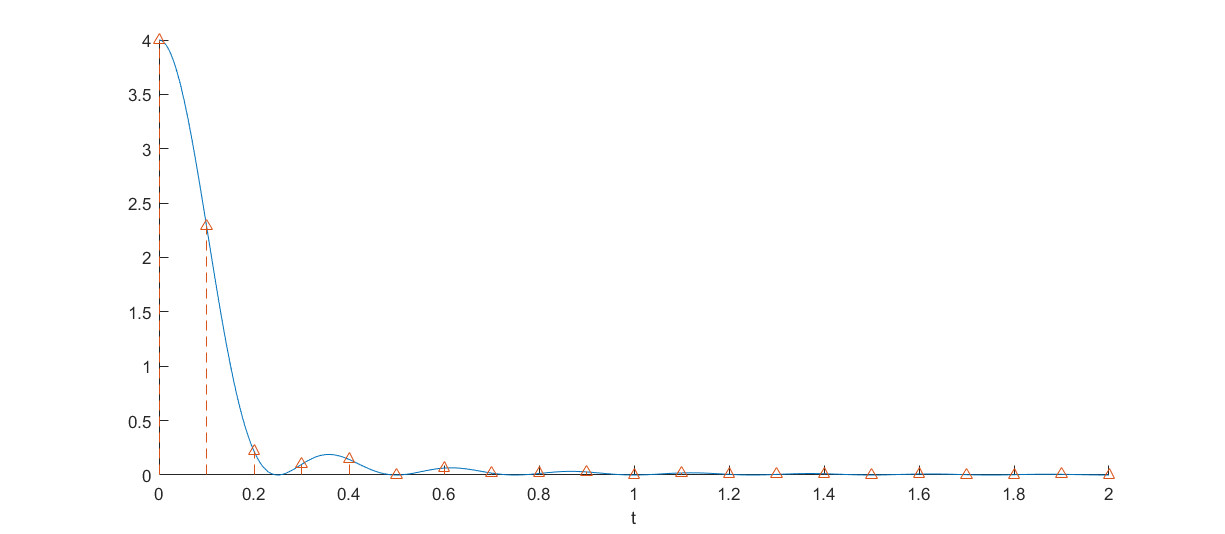
\includegraphics[width=0.7\textwidth]{figure.png}
	\caption{Signal $x(t)$ et $x_e[n]$}
	\label{fig:signal1}
\end{figure}
\begin{figure}
	\centering
	\begin{tikzpicture}[x=0.4cm, y=1.2cm]
	\draw[thick, -latex] (-15, 0) -- (15, 0);
	\draw[thick, -latex] (0, -1) -- (0, 1.8);
	\draw (16, -0.1) node[below] {$f$ (\si{\hertz})};
	\draw (0.1, 1) -- (-0.1, 1) node[left] {1};
	\draw (-14, 0.1) -- (-14, -0.1) node[below] {-14};
	\draw (-10, 0.1) -- (-10, -0.1) node[below] {-10};
	\draw (-6, 0.1) -- (-6, -0.1) node[below] {-6};
	\draw (-4, 0.1) -- (-4, -0.1) node[below] {-4};
	\draw (1, 0.1) -- (1, -0.1) node[below] {1};
	\draw (4, 0.1) -- (4, -0.1) node[below] {4};
	\draw (6, 0.1) -- (6, -0.1) node[below] {6};
	\draw (10, 0.1) -- (10, -0.1) node[below] {$f_e=$10};
	\draw (14, 0.1) -- (14, -0.1) node[below] {14};
	\draw[Green]
	(-10, -0.7) node {$-\omega_e=-20\pi$}
	(-4, -0.7) node {$-M = -8\pi$}
	(1, -0.7) node {$2\pi$}
	(4.1, -0.7) node {$M = 8\pi$}
	(10, -0.7) node {$\omega_e=2\pi f_e=20\pi$};
	\draw[Green] (16, -0.7) node {$\omega$ (\si{\radian\per\second})};

	\draw[Blue]
	(-10, -1.1) node {$-\Omega_e = -2\pi$}
	(-4, -1.1) node {$-0.8\pi$}
	(1, -1.1) node {$\frac{2\pi}{T_e}$}
	(4, -1.1) node {$0.8\pi$}
	(10, -1.1) node {$\Omega_e = 2\pi$};
	\draw[Blue] (16, -1.1) node {$\Omega$};

	\draw[Red]
	(-10, -1.4) node {$k=-N=-10$}
	(-4, -1.4) node {$k=-4$}
	(1, -1.4) node {$k=1$}
	(4, -1.4) node {$k=4$}
	(10, -1.4) node {$k=N=10$};
	\draw[Red] (16, -1.4) node {$k$};

	\draw[very thick] (-4, 0) -- (0, 1) -- (4, 0);
	\draw (-14, 0) -- (-10, 1) -- (-6, 0);
	\draw (6, 0) -- (10, 1) -- (14, 0);
	% DFT
	\draw[thin, Red, dashed]
	(0, 0) -- (0, 1) node {$\circ$}
	(1, 0) -- (1, 0.75) node {$\circ$}
	(2, 0) -- (2, 0.5) node {$\circ$}
	(3, 0) -- (3, 0.25) node {$\circ$}
	(4, 0) node {$\circ$}
	(5, 0) node {$\circ$}
	(6, 0) node {$\circ$}
	(7, 0) -- (7, 0.25) node {$\circ$}
	(8, 0) -- (8, 0.5) node {$\circ$}
	(9, 0) -- (9, 0.75) node {$\circ$};
	\draw[very thick] (5, 1.5) node {\textbf{FT de $x_\delta(t)$}};
	\draw (5, 1.2) node {FT de $x(t)$};
	\draw[Blue] (5, 0.9) node {DTFT de $x_e[n]$};
	\draw[Red] (5, 0.6) node {DFT de $x_e[n]$};
	\end{tikzpicture}
	\caption{Spectres du signal~\ref{fig:signal1}. $N=10$ et $f_e=10$ aussi. C'est évidemment un hasard ;-).}
	\label{fig:spectra1}
\end{figure}

A quoi ça ressemble tout ça ? La figure~\ref{fig:signal1} montre un signal
\[ x(t) = \frac{1-\cos(M t)}{\pi M t^2} \]
avec $M=2\pi \cdot 4$, dont la transformée est exactement
\[ X(j\omega) = \begin{cases}
1 + \frac{\omega}{M} & \text{si } -M \le \omega \le 0 \\
1 - \frac{\omega}{M} & \text{si } 0 < \omega \le M \\
0 & \text{sinon}
\end{cases} \]
ainsi que le signal $x_\delta(t)$, résultat de l'échantillonnage de $x(t)$ à une fréquence de $f_e = \SI{10}{\hertz}$. La figure~\ref{fig:spectra1} présente la transformée du signal de départ (en gras), ainsi que deux des répliques du signal $x_\delta(t)$ après échantillonnage.

La DTFT de $x_e[n]$ et la FT de $x_\delta(t)$ ne diffèrent que par l'échelle en fréquence, et se superposent parfaitement quand on prend deux échelles telles que $\Omega = \omega T_e$. Pour information, le $2\pi$ vert en dessous de 1 provient de $\frac{2\pi}{N T_e}$ avec $N=10$ et $T_e=0.1$.

\begin{figure}
	\centering
	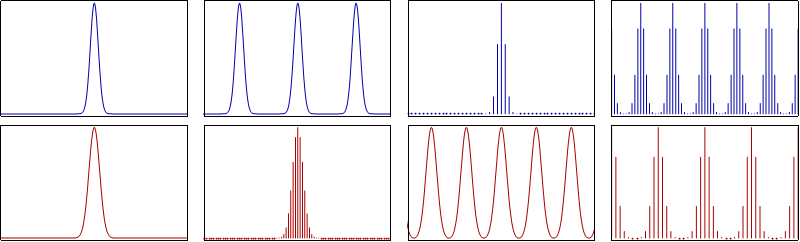
\includegraphics[width=0.8\textwidth]{From_Continuous_To_Discrete_Fourier_Transform.png}
	\caption{Un autre exemple}
	\label{fig:signalspectra2}
\end{figure}
\begin{figure}
	\centering
	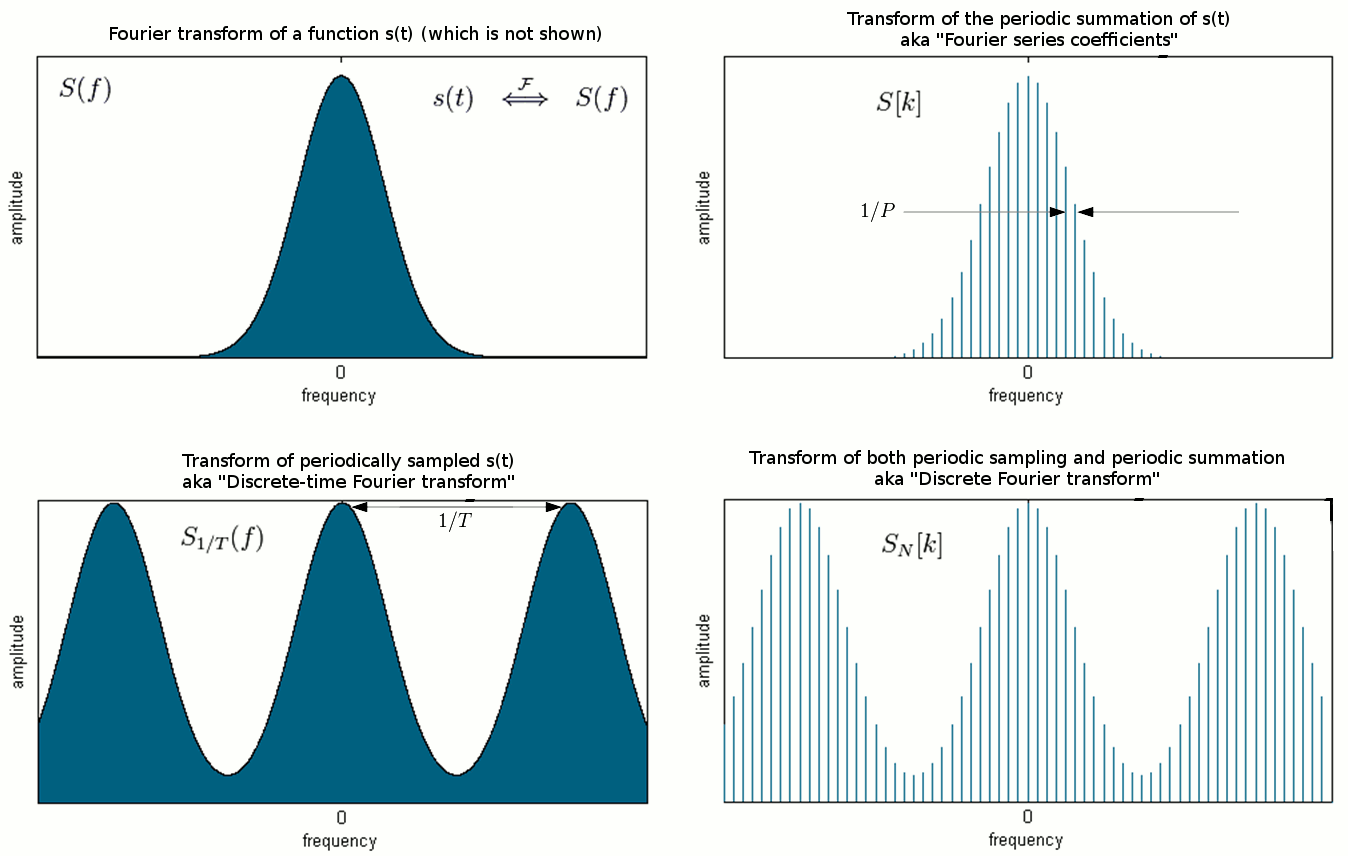
\includegraphics[width=0.8\textwidth]{Fourier_transform,_Fourier_series,_DTFT,_DFT.png}
	\caption{Un autre exemple, très proche du deuxième}
	\label{fig:signalspectra3}
\end{figure}

Les figures~\ref{fig:signalspectra2} et~\ref{fig:signalspectra3}, venant de Wikipedia, montrent la même chose, mais peut-être en plus propre.

Dans la première figure, les graphes du dessus sont les signaux, dans les domaines temporels et discrets ($t$ et $n$), et les graphes du dessous sont les spectres, dans les domaines fréquentiels ($\omega$, $\Omega$, $f$ et $k$) ; chaque spectre correspond au signal du dessus.

Le premier signal est notre signal de départ, $x(t)$, avec sa FT $X(j\omega)$ ; les deux sont parfaitement continus. Le deuxième est le résultat de l'échantillonnage de la FT, qui produit donc une FS $\hat{X}[k]$ mais qui rend aussi le signal de départ $T$-périodique (appelons-le $x_P(t)$). Le troisième signal est l'échantillonnage $x_e[n]$, qui se fait à fréquence $f_e$ (ou $\omega_e=2\pi f_e=\frac{2\pi}{T_e}$) ; le spectre devient alors $\omega_e$-périodique (FT $X_\delta(j\omega)$), ou $2\pi$-périodique (DTFT $X\left(e^{j\Omega}\right)$). Enfin, le quatrième graphe est la combinaison des deux échantillonnages : notre signal $x(t)$ a finalement été transformée en un signal discret $x_N[n]$, qui est $N$-périodique (et qui ressemble au signal $T$-périodique $x_P(t)$), et le spectre est lui aussi discret et $N$-périodique.

Dans la deuxième figure, le signal en temporel n'est pas montré. On reconnait, de gauche à droite et de haut en bas, la FT $X(j\omega)$ originale, la FS $\hat{X}[k]$, la DTFT $X_e\left(e^{j\Omega}\right)$\footnote{ou la FT $X_\delta(j\omega)$}, et la DFT $X[k]$. Sur le diagramme, les fréquences sont en hertz, avec $f$, au lieu de $\omega$ en radians par seconde ; $1/T$ est la fréquence d'échantillonnage (à la place de $1/T_e$) ; $P$ est la période du signal $x_P(t)$ (la version périodisée de $x(t)$) (à la place de $T$).

\begin{figure}
	\centering
	\includegraphics[width=0.75\textwidth]{no-zeropad.png}
	\caption{Sans zero-padding}
	\label{fig:nozeropadding}
\end{figure}
\begin{figure}
	\centering
	\includegraphics[width=0.8\textwidth]{zeropad.png}
	\caption{Avec zero-padding}
	\label{fig:zeropadding}
\end{figure}

Encore un exemple, cette fois de l'importance du \emph{zero-padding}. Considérons un signal $x[n] = e^{\frac{2j\pi n}{8}}$, pour $n=0,\dots,L-1$ avec $L=64$, et $0$ sinon. C'est donc un signal non périodique, de durée finie, qui a une DTFT qui ressemble à un $\mathrm{sinc}$.

Si on prend la DFT de ce signal, en utilisant exactement les $N=L=64$ échantillons non nuls, on obtient la figure~\ref{fig:nozeropadding} : le signal a été considéré comme étant périodique par la DFT, ce qui est logique, vu que sur ces $64$ échantillons, le signal est parfaitement périodique ($64$ est un multiple de la période du signal, $8$). En fait, si le signal avait été périodique et infini, alors la DTFS nous aurait donné le même signal.

Si on prend la DFT de ce signal, en utilisant cette fois $N=256$ échantillons, avec $192$ échantillons nuls pour combler, on obtient la figure~\ref{fig:zeropadding}, bien plus proche de la DTFT vraie de ce signal. Les échantillons supplémentaires nuls ont forcé la DFT à considérer que ce signal est non périodique, et il ne s'est donc pas trompé lors du calcul : on a presque la bonne DTFT.

A noter que la DFT obtenue sans zero-padding reste un échantillonnage de la vraie DTFT : elle a simplement sélectionnée des échantillons nuls partout sauf à la fréquence du début du signal. La DTFT de ce signal s'annule, de manière coïncidente\footnote{Mais démontrable.}, à 64 endroits équidistants sur toute la période, sauf à un endroit : là où est la fréquence du morceau non nul du signal.

\end{document}
